%Structural Biology
Over the past century, elucidating the three-dimensional (3D) structures of macromolecules has fundamentally enriched our understanding of biochemistry,\cite{Shi2014, Wagner1997} creating the field of structural biology. Achievements like the structure of deoxyribonucleic acid (DNA)\cite{Watson1953} (with the unpublished work of Rosalind Franklin\cite{Elkin2003}) led to the central dogma of molecular biology \cite{Crick1970}, while the first structure of an $\alpha$-helix \cite{Pauling1951} shaped our understanding of the structural building blocks in protein structures. Over time, various methods have been developed to elucidate 3D structures, with the most prominent methods being X-ray crystallography\cite{Ladd1977, Shi2014}, nuclear magnetic resonance (NMR),\cite{Wagner1997,  Shi2014, Jacobsen2007, Markwick2008} and the more recent single-particle cryo-electron microscopy\cite{Doerr2016, Agard2014, Cheng2017, Kuhlbrandt2014}. The first complete 3D structure of a protein was of myoglobin\cite{Kendrew1958}, published in 1958, opening the door for molecular modeling with biomolecules and rational drug design.
%% MD sims with biochem. first applications
Early perspectives on proteins considered their structure to be very rigid.  \cite{Karplus2002} This belief was transformed to a much more dynamic understanding of protein structures, influenced by theoretical methods such as molecular dynamics (MD) simulations \cite{Karplus2002, Phillips1981} and by developments in experimental methodology, e.g., the B-factor analysis for X-ray crystallography\cite{Frauenfelder1979} and NMR \cite{Wuthrich1975, Torchia1984, Dobson1986}. The first MD simulation contributing to the transition was performed by McCammon \textit{et al.} on the pancreatic trypsin inhibitor (BPTI) for $9.2~ps$ under vacuum conditions. \cite{Mccammon1977} 

%%Examples of application
To date, a considerable amount of literature has been published using MD simulations to model the conformational behavior of biological systems containing proteins, nucleic acids, carbohydrates, and lipid membranes. \cite{Leach2001, Karplus2002, Chavent2014, Hollingsworth2018} In these studies, simulation techniques are used to support structure determination, or to provide insights on thermodynamic or kinetic quantities. \cite{Gunsteren1990, Karplus2002} 
Often, a combination of theoretical and experimental methods is used to exploit the complementary nature of the techniques and their synergies. \cite{Gunsteren2008} An example for such a combined approach is given in Chapter \ref{ch:cycpep}, where a rational for the difference in membrane permeability due to a stereocenter change in macrocyclic compounds   is obtained based on MD simulation results,  validated by additional experimental NMR.

%Thermodynamic quantities
With the first concept for binding free-energy calculations using MD simulations by Tembre\cite{Tembre1984}, an important step toward rational drug design was made. \cite{Durrant2011}
However, this scheme for absolute free-energy calculations proved to be computationally very expensive and therefore was not feasible for a long time. Only relatively recently, advances in computer hardware and methodology have started to overcome these barriers. \cite{Chodera2011, Aldeghi2016}
Another important step toward rational drug design was made by Jorgensen and co-workers with the first relative free-energy calculation, opening the field to a more efficient methodology.\cite{Jorgensen1988, Chodera2011} 
Today, free-energy calculations are (becoming) a standard tool in the drug discovery process and support the design of modern therapeutics. \cite{Chodera2011, Christ2014,  Cournia2017, Cournia2020, Jorgensen1983, Meier2021}
 
Ligand binding free energies are not the only properties of interest for drug design. Another aspect that gained coverage recently in computational literature is the passive membrane permeability of drug molecules, as discussed in Chapter \ref{ch:cycpep}. \cite{Witek2016, Witek2017, Witek2019,  Wang2021, Marrink1996, Bemporad2004, Sugita2021, Corbett2021} 
As simulations can nowadays routinely reach timescales in the order of $\mu$s, conformational dynamics can be determined to provide insight into the kinetic behavior of molecules.\cite{Witek2016, Witek2017} In this context, a particular interest lies in compound that are beyond the Lipinksi\cite{Lipinski2001} rule-of-5.\cite{Witek2016, Witek2017, Witek2019,  Wang2021, Sugita2021} These more complex molecules such as the cyclic peptide cyclosporin A explore a larger conformational space. The good membrane permeability of cyclosporin A is hypothesized to be due to its chameleonic nature, allowing the molecule to adopt closed (apolar) and open (polar) conformations depending on the polarity of the environment.\cite{Witek2016, Witek2017}

A short introduction to simulation techniques and free-energy calculations is provided in the next section.

\section{Molecular Dynamics Simulations}
MD simulations are powerful tools that enable the study of biomolecular systems under certain conditions. Four aspects of simulations will be shortly discussed: the model, force fields and interaction functions, integration schemes, and simulation conditions.

\subsection{Model}
In computational chemistry, simulations provide information about molecules and their properties. Three different levels of resolution are usually distinguished.\cite{Barros2022}
The highest resolution is based on quantum mechanics (QM) with an explicit description of the electrons.\cite{Senn2009} Simulations on this level can for example provide insights into enzymatic reactions \cite{Sheng2020, Kazemi2015, Ryde2003,Naray2003} or photon-induced electron excitation\cite{Rivera2019, Li2008, Askerka2017}.  

The next lower level is molecular mechanics (MM), which is based on classical mechanics with atoms as single particles. Such atomistic simulations enable insights into the conformational behavior of molecules, \cite{Witek2016, Wang2021, Schenkmayerova2021, Mccammon1977} reaching much longer simulation times compared QM calculations. Note that this difference in computational cost led to the development of hybrid QM/MM methods, which are frequently used in modeling enzymatic reactions.\cite{Senn2009}
The third, most approximate level is called coarse-grained (CG), where multiple atoms or even multiple molecules are described by CG beads.\cite{Tozzini2005} Simulations on this level can access even longer timescales, enabling the study of polymer formation \cite{Hyeon2011, Shen2009} or crowding effects in cells\cite{Hong2020, Friedel2003}. 

In practical terms, the choice of a model defines the resolution of the coordinate and topology space of a system, which in turn specifies the phenomena that can be studied. In this thesis, the theory level of choice is MM with the united atoms approach\cite{Daura1998} for aliphatic CH$_X$ groups. 

\subsection{Force Fields and Interaction Functions}
Empirical research has led to rules and concepts for atoms and their interactions with each other, for example covalent bond lengths and electrostatic interactions.\cite{Morse1929, Pauling1934, Gillmor2017} 
Interaction functions are used in modeling to represent these empirical rules and concepts. The required function parameters can be retrieved directly from the system coordinates or provided via a predefined topology.  \cite{Mackerell2004, Cornell1995, Oostenbrink2004} 
Topological parameters are often inferred from higher-level theoretical approaches such as QM, or fitted to reproduce experimental properties. \cite{Oostenbrink2004}

\begin{figure}[h!]
    \centering
    \begin{subfigure}{0.45\textwidth}
        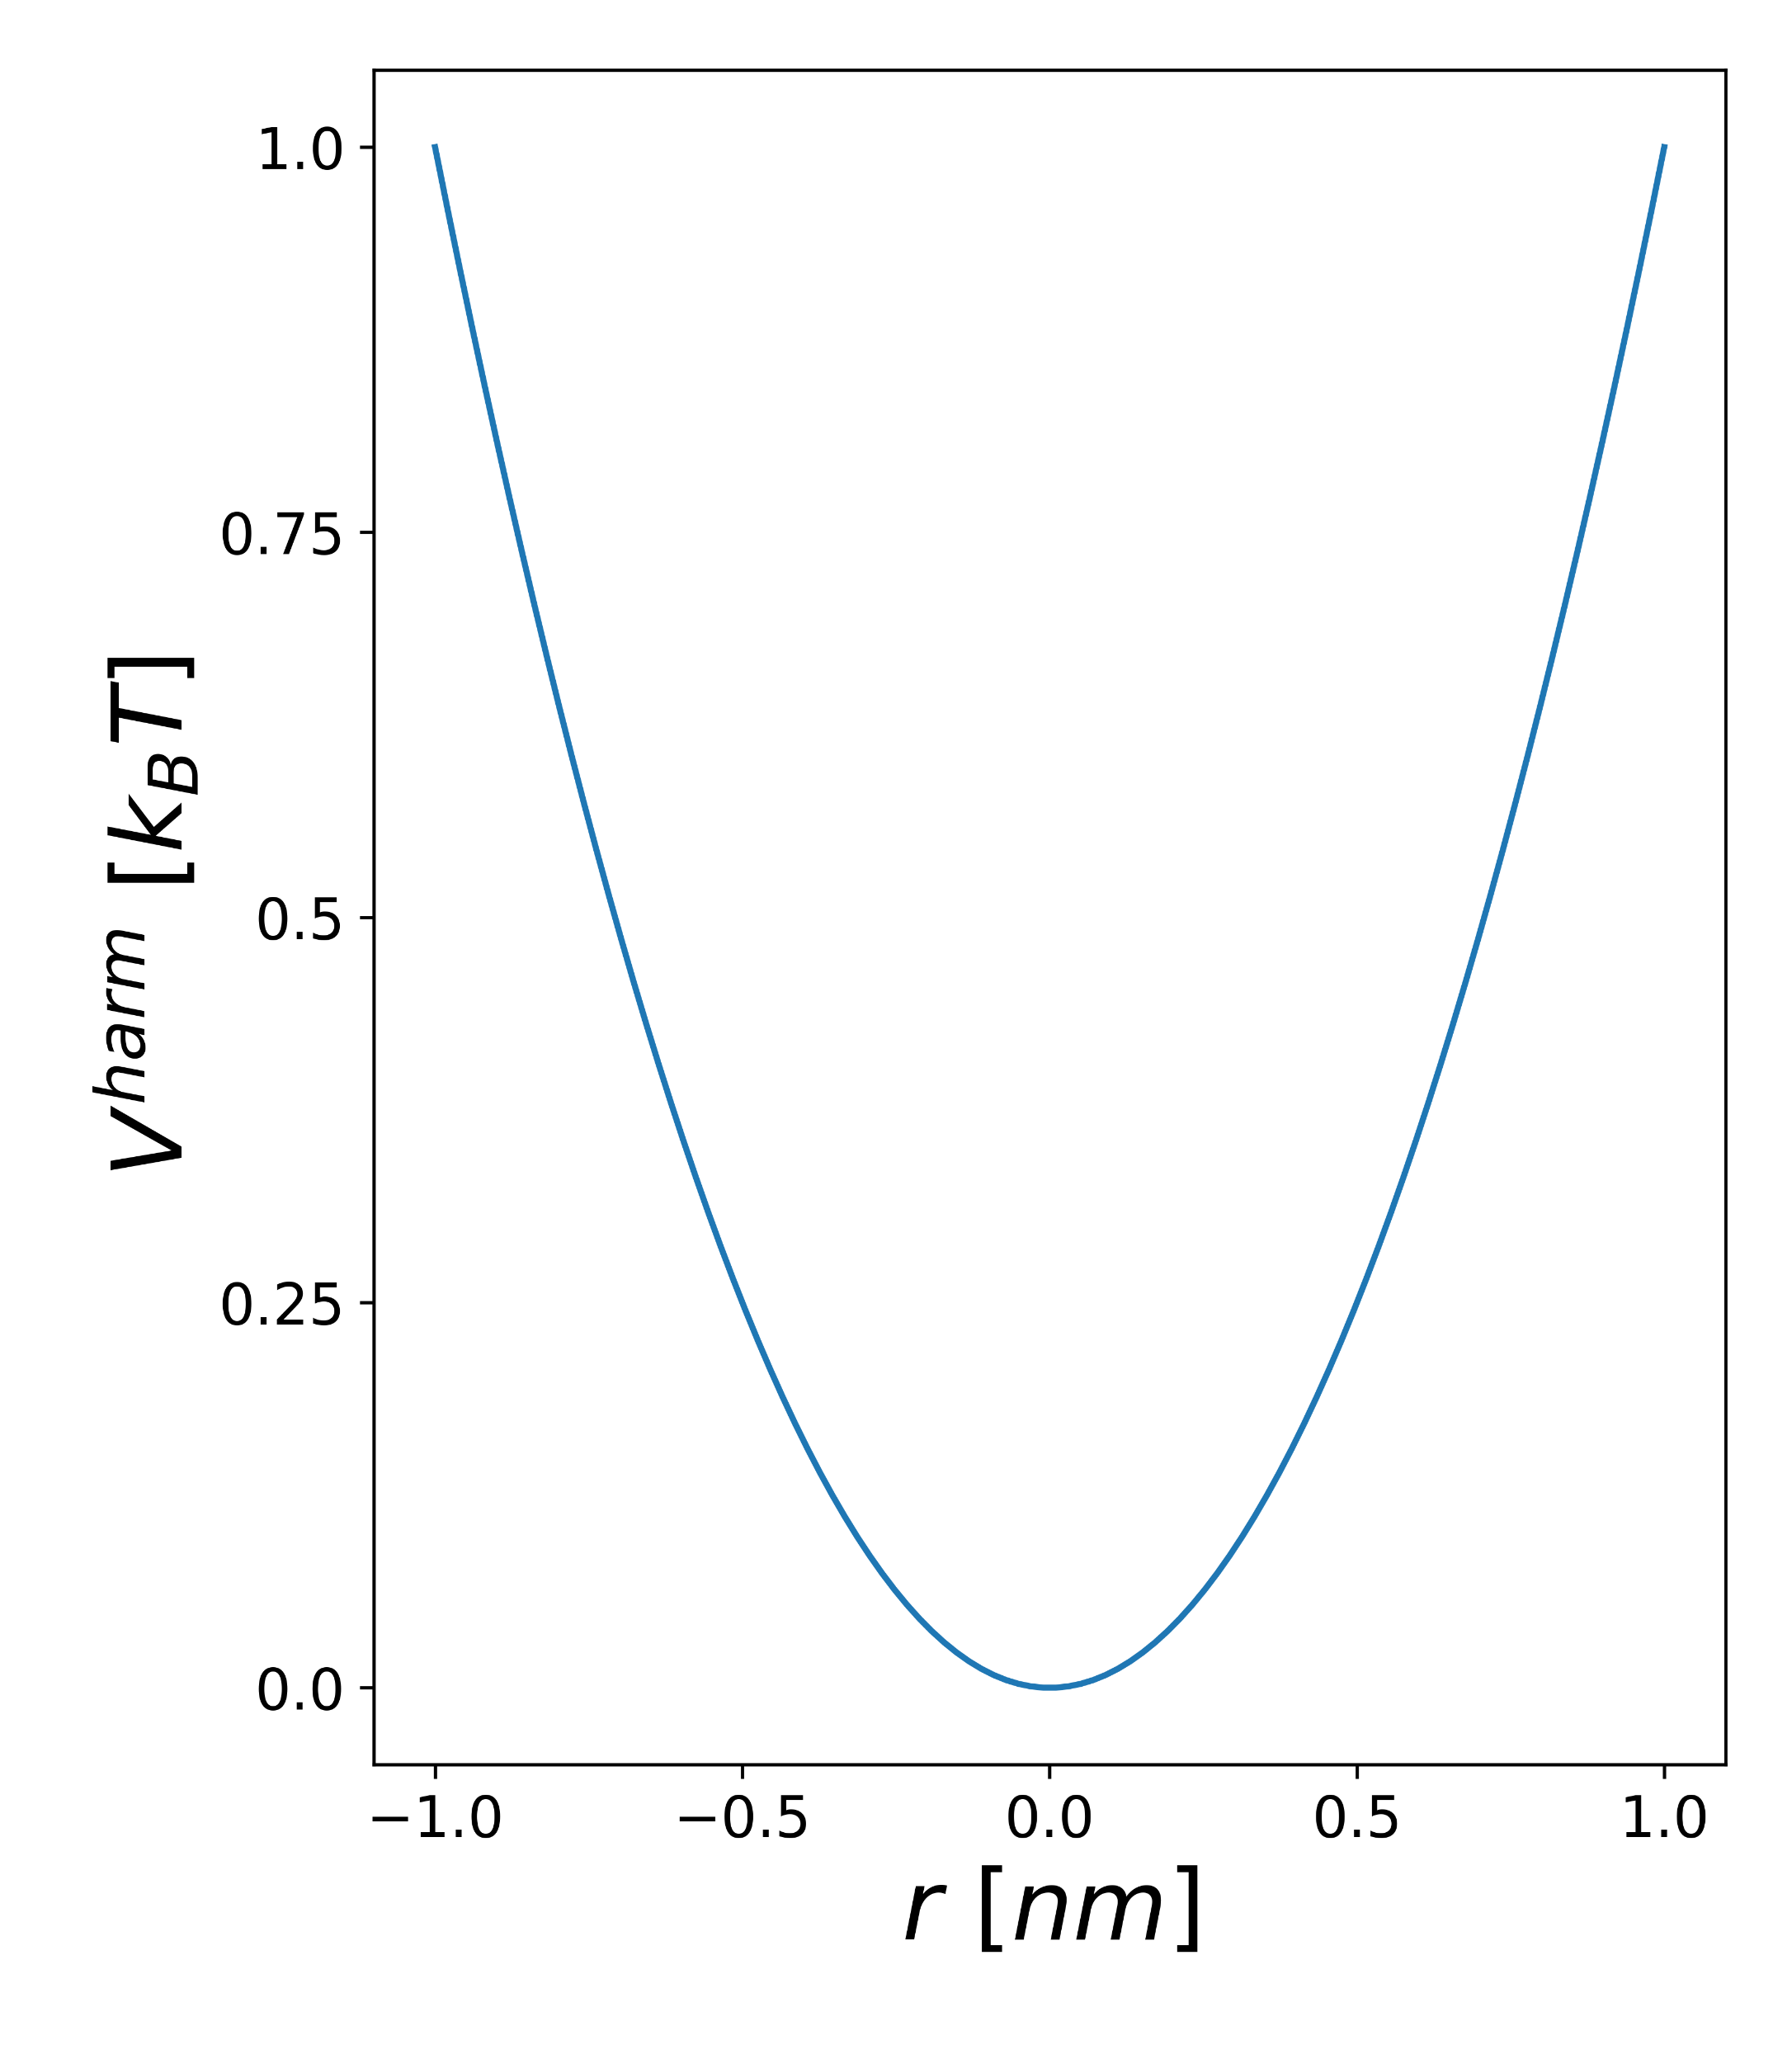
\includegraphics[width=\textwidth]{2_chapter_intro/fig/ForceField/harmOscV.png}
        \caption{Harmonic Oscillator}
	\label{sfig:ho}
    \end{subfigure}
        \begin{subfigure}{0.45\textwidth}
        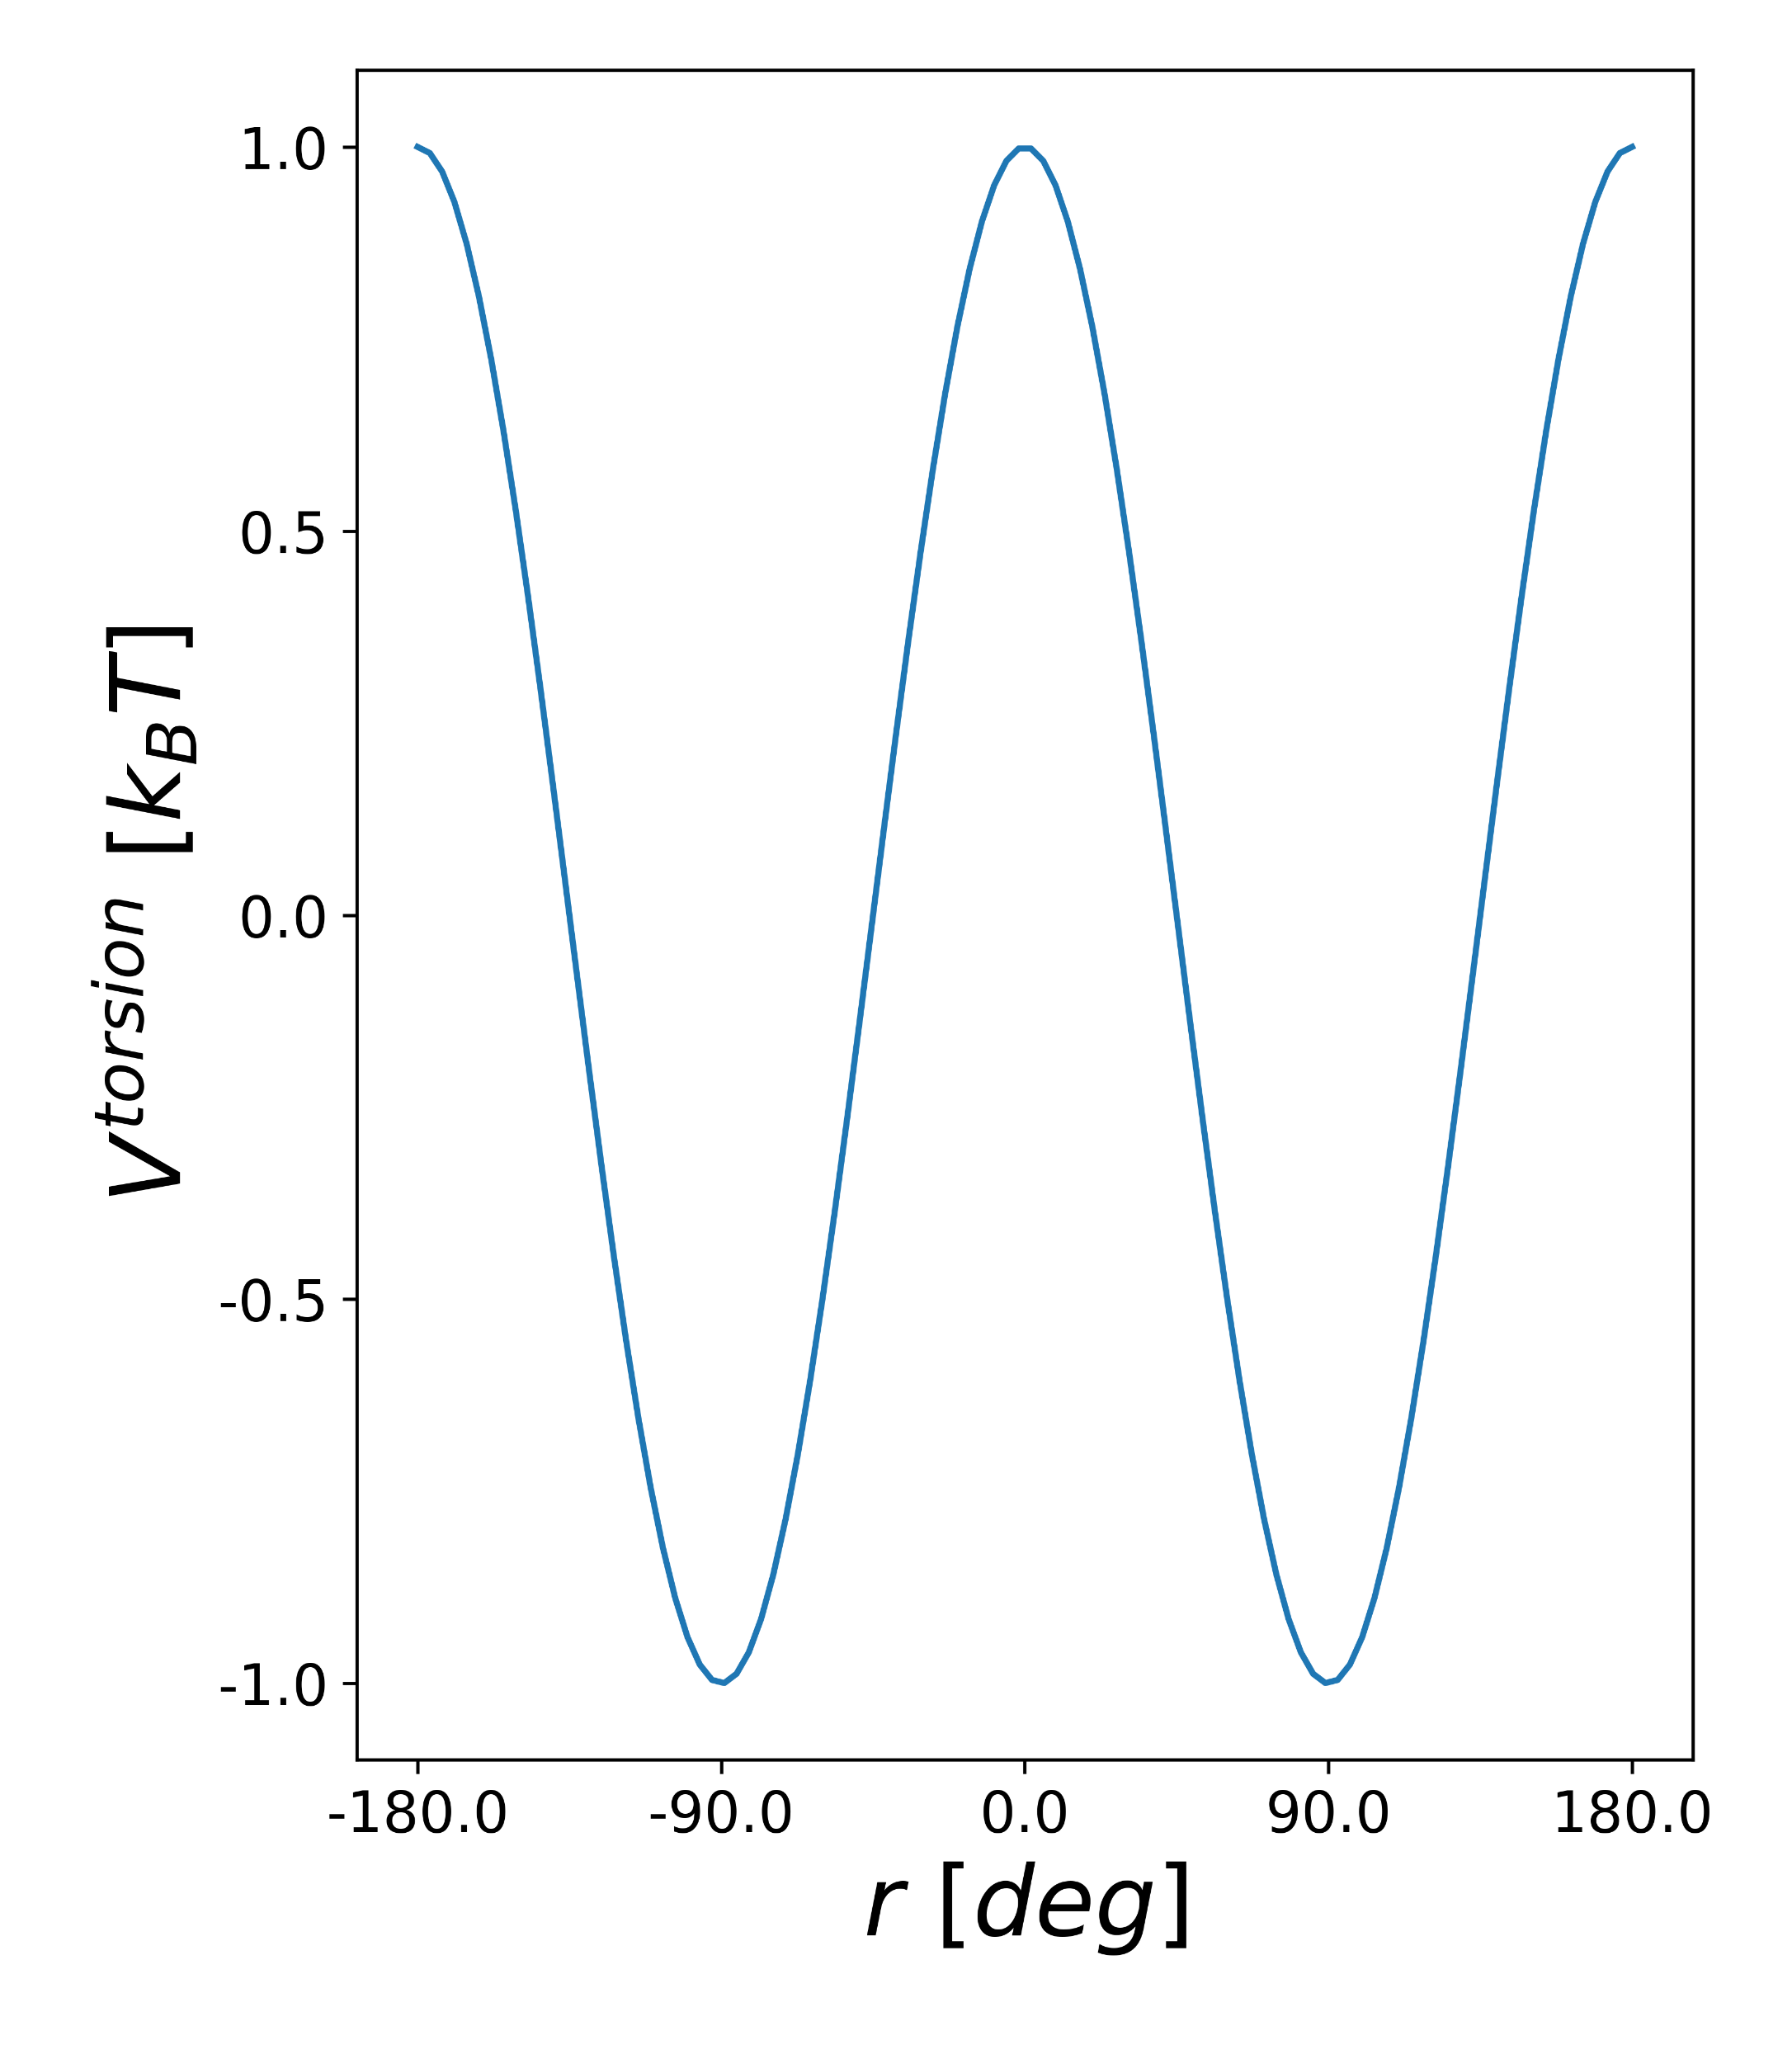
\includegraphics[width=\textwidth]{2_chapter_intro/fig/ForceField/torsV.png}
        \caption{Trigonometric potential Function}
	\label{sfig: tf}
    \end{subfigure}
    \\
        \begin{subfigure}{0.45\textwidth}
        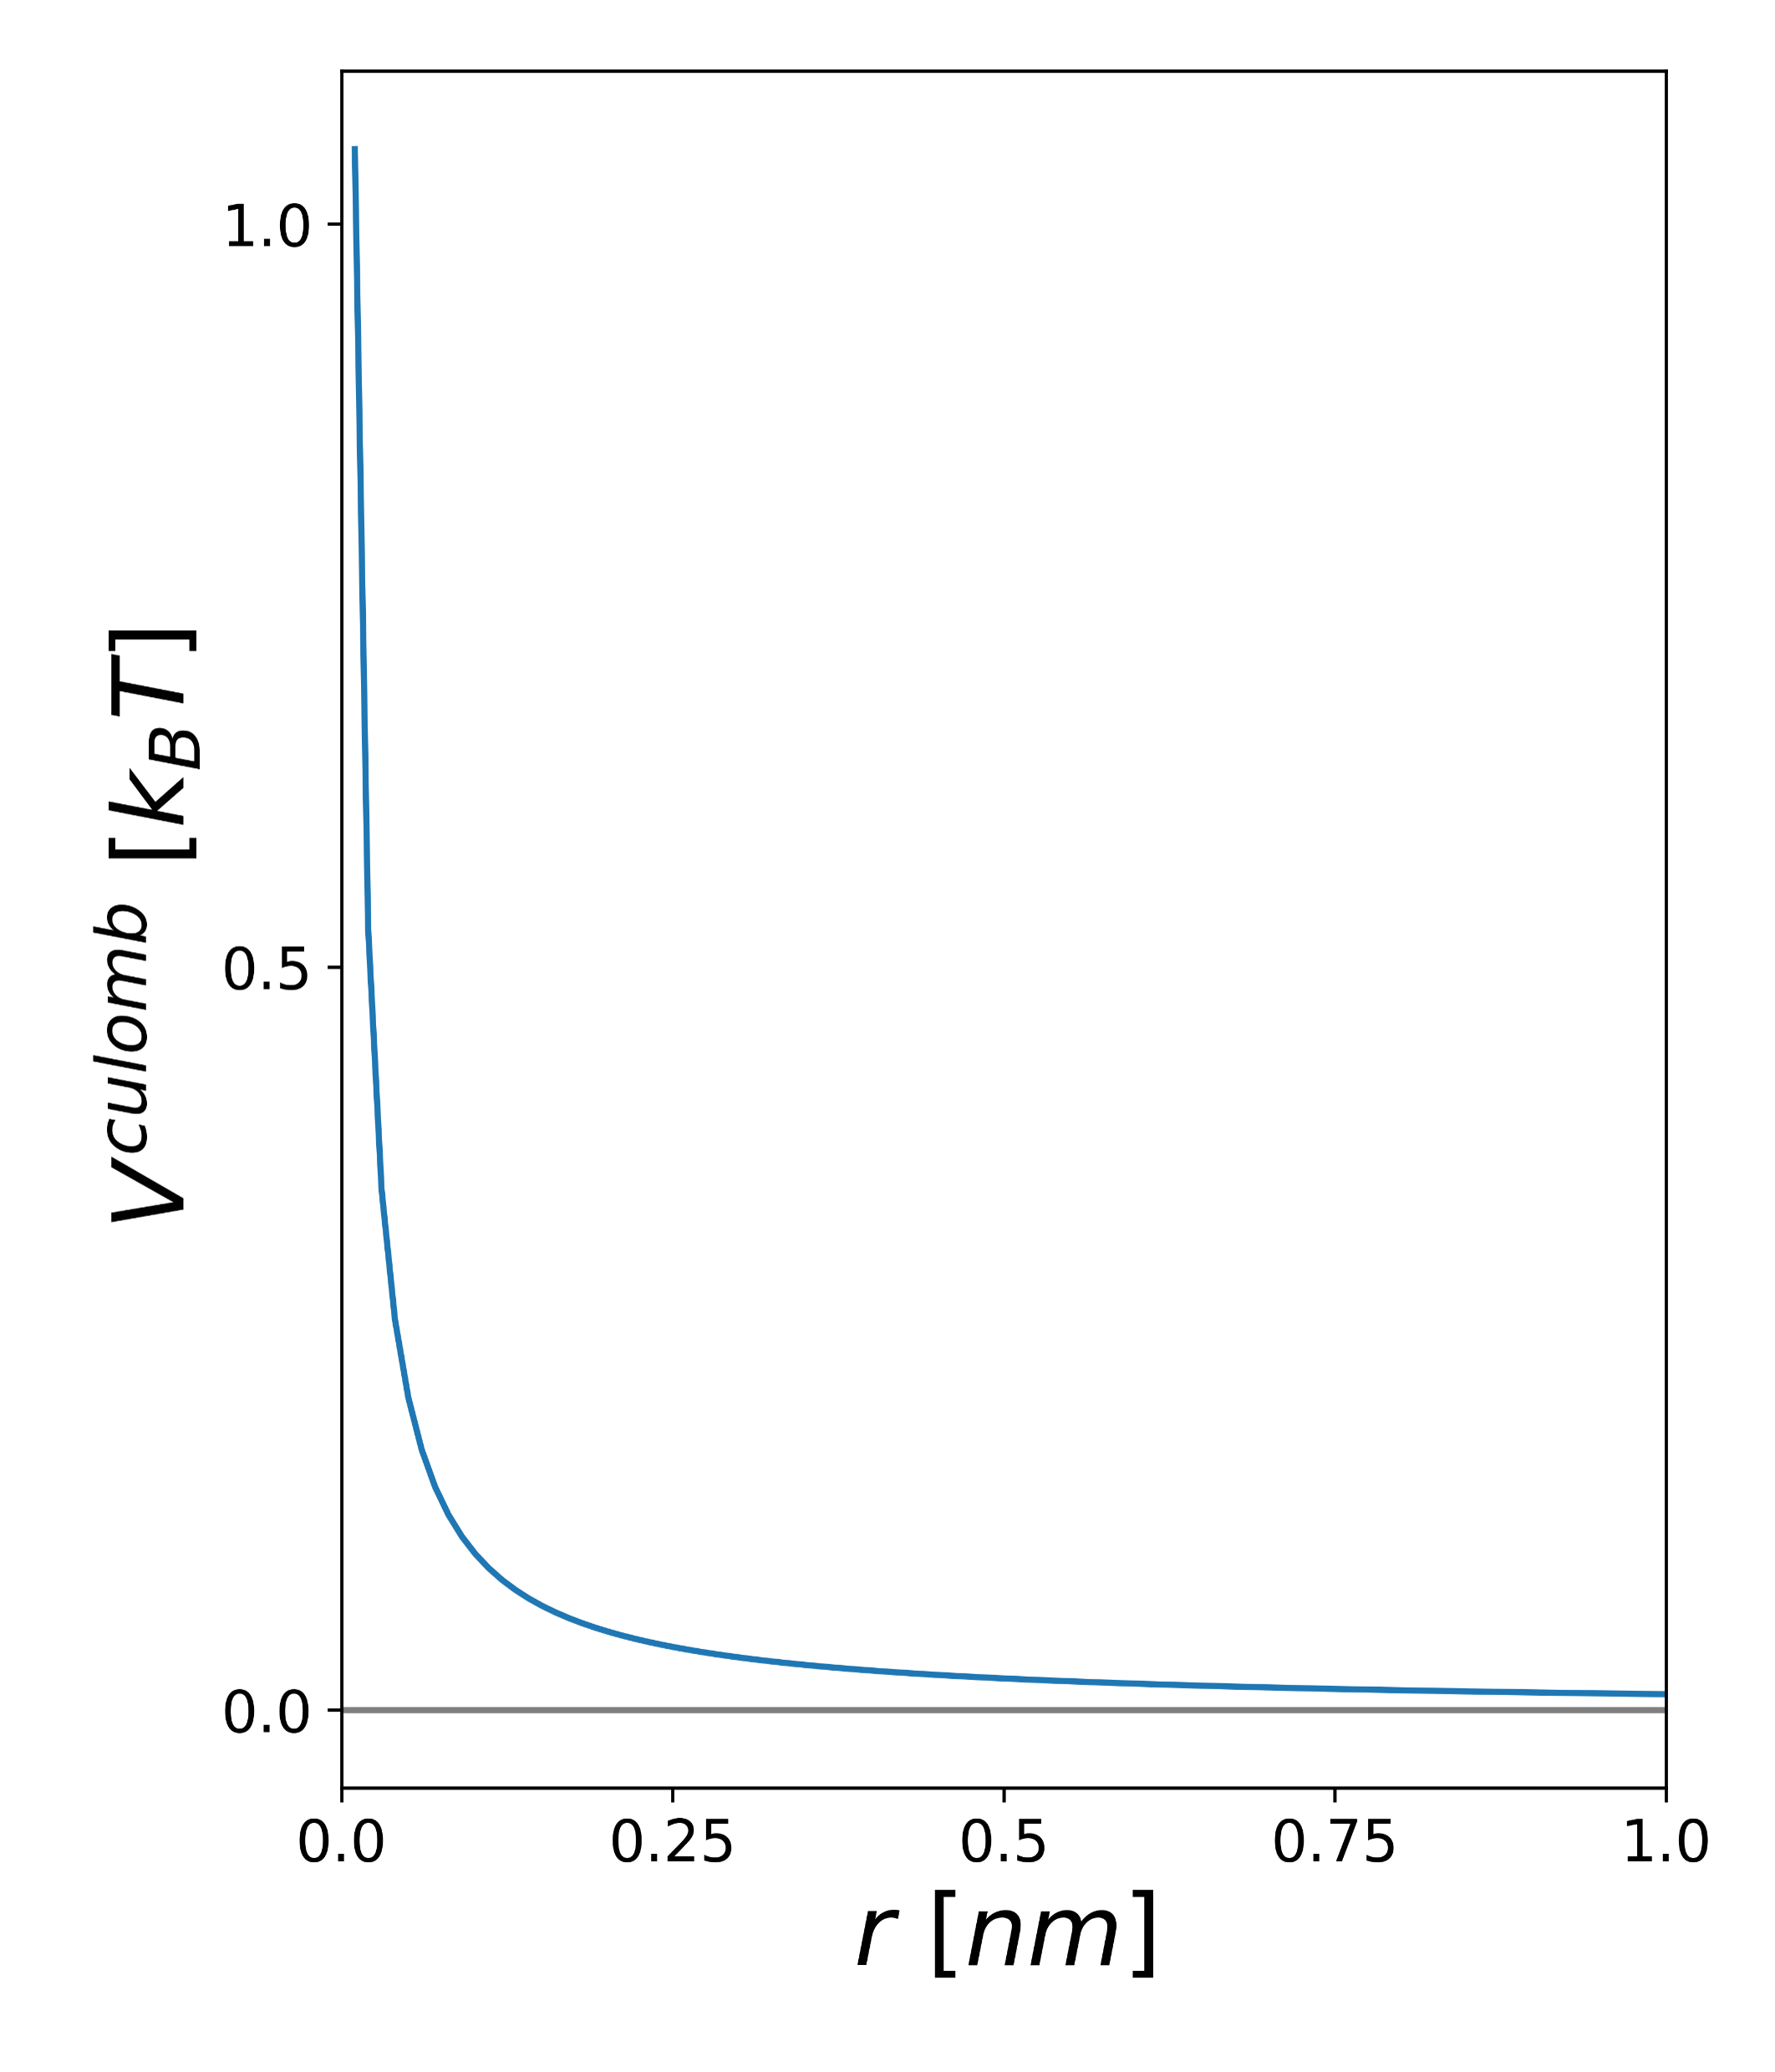
\includegraphics[width=\textwidth]{2_chapter_intro/fig/ForceField/coulombV.png}
        \caption{Coulomb potential function}
	\label{sfig: cf}
    \end{subfigure}
        \begin{subfigure}{0.45\textwidth}
        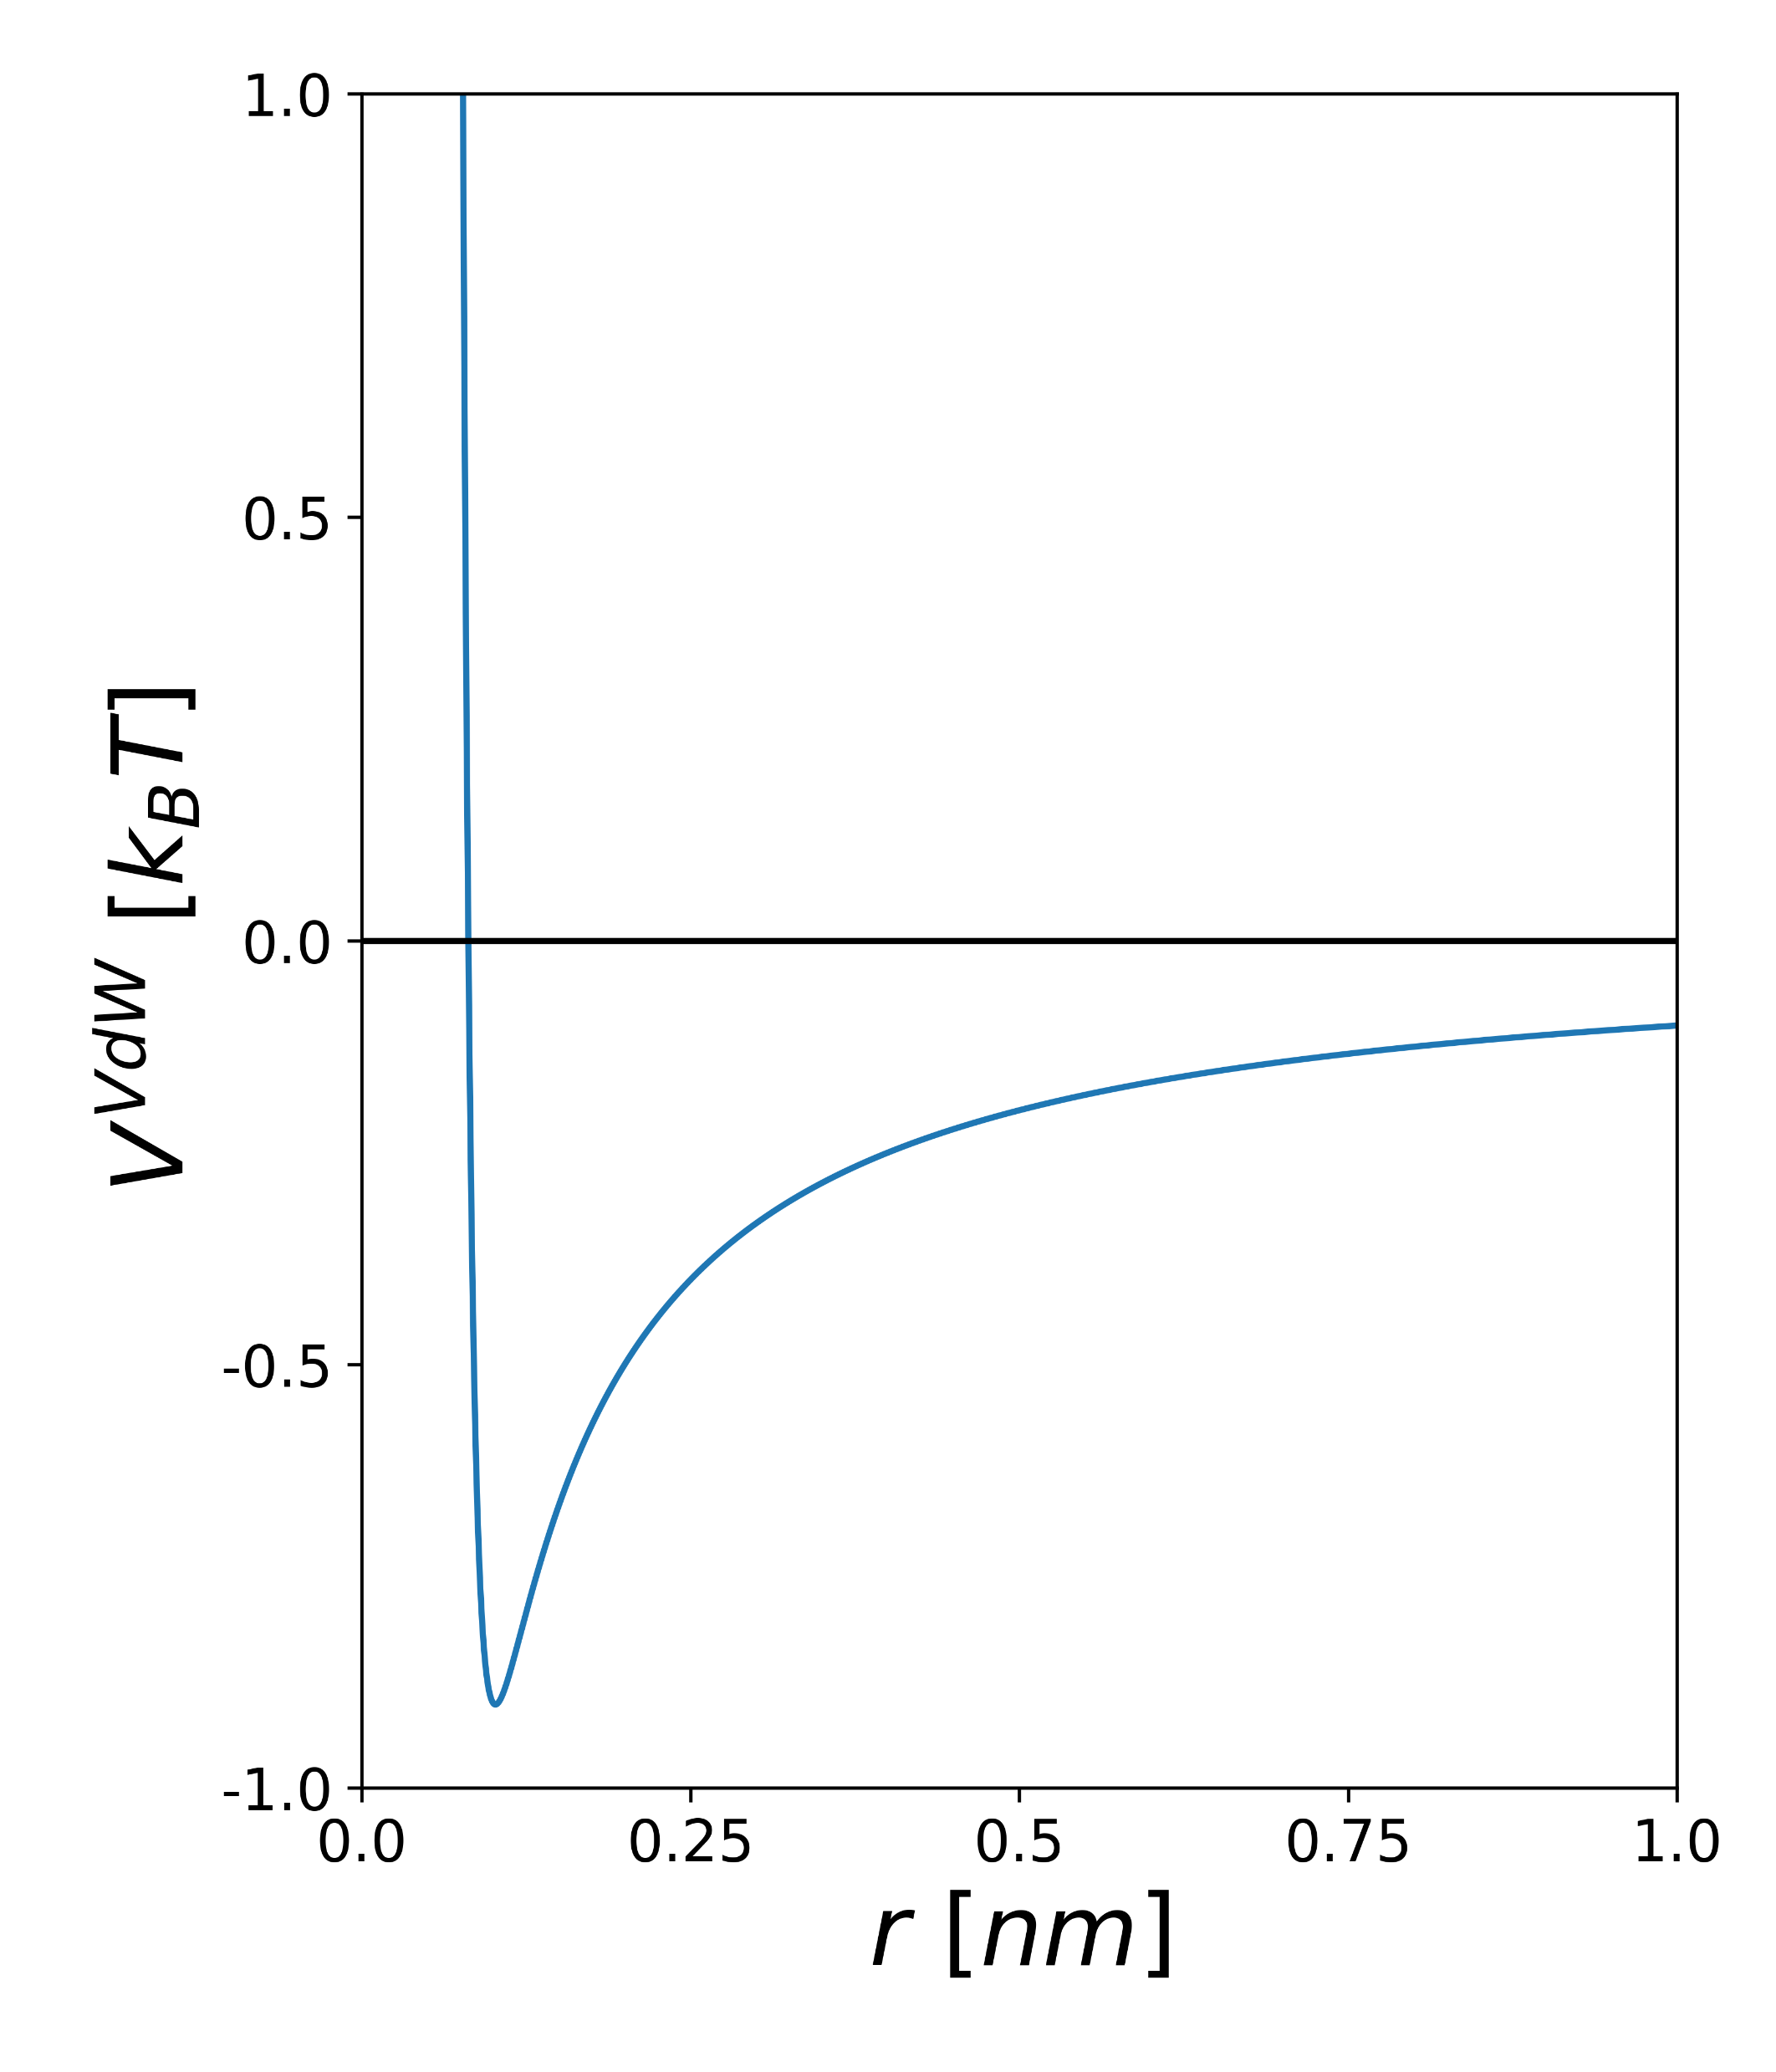
\includegraphics[width=\textwidth]{2_chapter_intro/fig/ForceField/vdwV.png}
        \caption{Lennard Jones 6-12}
	\label{sfig: lj}
    \end{subfigure}
    \caption{Potential-energy functions to represent atom--atom interactions. (A): Covalent bond stretching, bond angle bending and improper dihedral. (B): Torsion dihedral angle. (C): Electrostatic interaction, modelled by a Coulomb potential-energy function. (D): Wan der Waals interactions, modelled by a Lennard Jones potential-energy function.}
    \label{fig:FF_Functions}
\end{figure}

The interaction functions can be split into two classes: (i) the intramolecular bonded terms and the intermolecular interactions nonbonded terms. \cite{Oostenbrink2004}
The following interaction types are relevant in this thesis for the bonded terms: Covalent bond stretching, bond angle bending and bond dihedral angle rotation.
Covalent bonds of two atoms are an essential part of chemistry to build up molecules. \cite{Pauling1934} The length of a bond and its stretching impact was famously described by the Morse potential function. \cite{Morse1929, Iozzi2009} However, in simulations, this bond stretching term is usually approximated with the less complex harmonic oscillator potential or alternative forms(Figure \ref{sfig:ho}).\cite{Oostenbrink2004} Bond angles can be calculated between three atoms. This property can be used, for example, to describe the tetraether conformation of sp3 hybridized carbon atoms ($\alpha = 109.5 \text{deg}$). \cite{Pauling1931, Slater1931} The same concept of harmonic oscillator potential functions is used to model the bond angle behavior (Figure \ref{sfig:ho}). \cite{Oostenbrink2004} 
The torsion (or dihedral) angle describes the rotation around a covalent bond. \cite{Blondel1996} It can be calculated from a set of four atoms and is an important quantity in chemistry that is fundamental for concepts like Cis and Trans isomerization \cite{Dugave2003} or ring conformations\cite{Strauss1970}. This property is modeled with trigonometric functions  (Figure \ref{sfig: tf}). \cite{Oostenbrink2004} 
Additionally, so-called improper dihedrals are applied to model rotation barriers, the functionals used for these interaction terms again being based on harmonic oscillators (Figure \ref{sfig:ho}). \cite{Oostenbrink2004,Blondel1996}

The class of nonbonded terms describes atom interactions depending on their spatial distance. Here two fundamental terms are commonly applied.
On the one hand, the electrostatic term describes the interaction of polar atoms with each other and is modeled by a Coulomb potential. \cite{Gillmor2017, Atkins2014} In standard MD simulation tools, a spatial cutoff limits the directly calculated coulomb terms for computational efficiency reasons. The introduced cutoff inaccuracies are compensated by expanding the interaction function by additional terms that describe the electrostatic environment contribution, like the reaction field method (RF) \cite{Tironi1995} or the particle mesh Ewald method (PME) \cite{Darden1993}.
On the other hand, the Van der Waals terms or dispersive interactions describe the electron fluctuations in atoms and their resulting interaction potential.\cite{Kawai2016, Margenau1939} The Van der Waals forces \cite{Margenau1939} are usually modeled with a Lennard Jones 6-12 potential \cite{Jones1924}. \cite{Oostenbrink2004}
From a computational perspective, calculating the nonbonded terms is usually the most computationally expensive operation. The complexity derives from the required distance calculation and amount of terms representing the interactions. However, these terms can be well parallelized to significantly speed up the calculation process.\cite{Berendsen1995, Schmid2012, Eastman2010, Meel2008}

Multiple interaction functions are summed up to a force field function (FF). The FF describes the total potential energy $V(\textbf{r})$ of a given coordinate set of a system $\textbf{r}$ and its atom interactions. 
\begin{equation}
\begin{split}
    V(\textbf{r}) &= V^{bonded}(\textbf{r}) + V^{nonbonded}(\textbf{r})\\
          &= V^{bond}(\textbf{r}) + V^{angle}(\textbf{r}) \\
          &~ + V^{torsion}(\textbf{r}) + V^{improper}(\textbf{r}) \\
          &~ + V^{electrostatics}(\textbf{r}) + V^{vdW}(\textbf{r})
\end{split}
\end{equation}
The total coordinate space gives rise to the potential energy surface (PES) defined by an FF (Figure \ref{fig:ffPES}).
During simulation, minima and barriers of the PES are explored and give insights into the conformational behavior of a system.

\begin{figure}
    \centering
    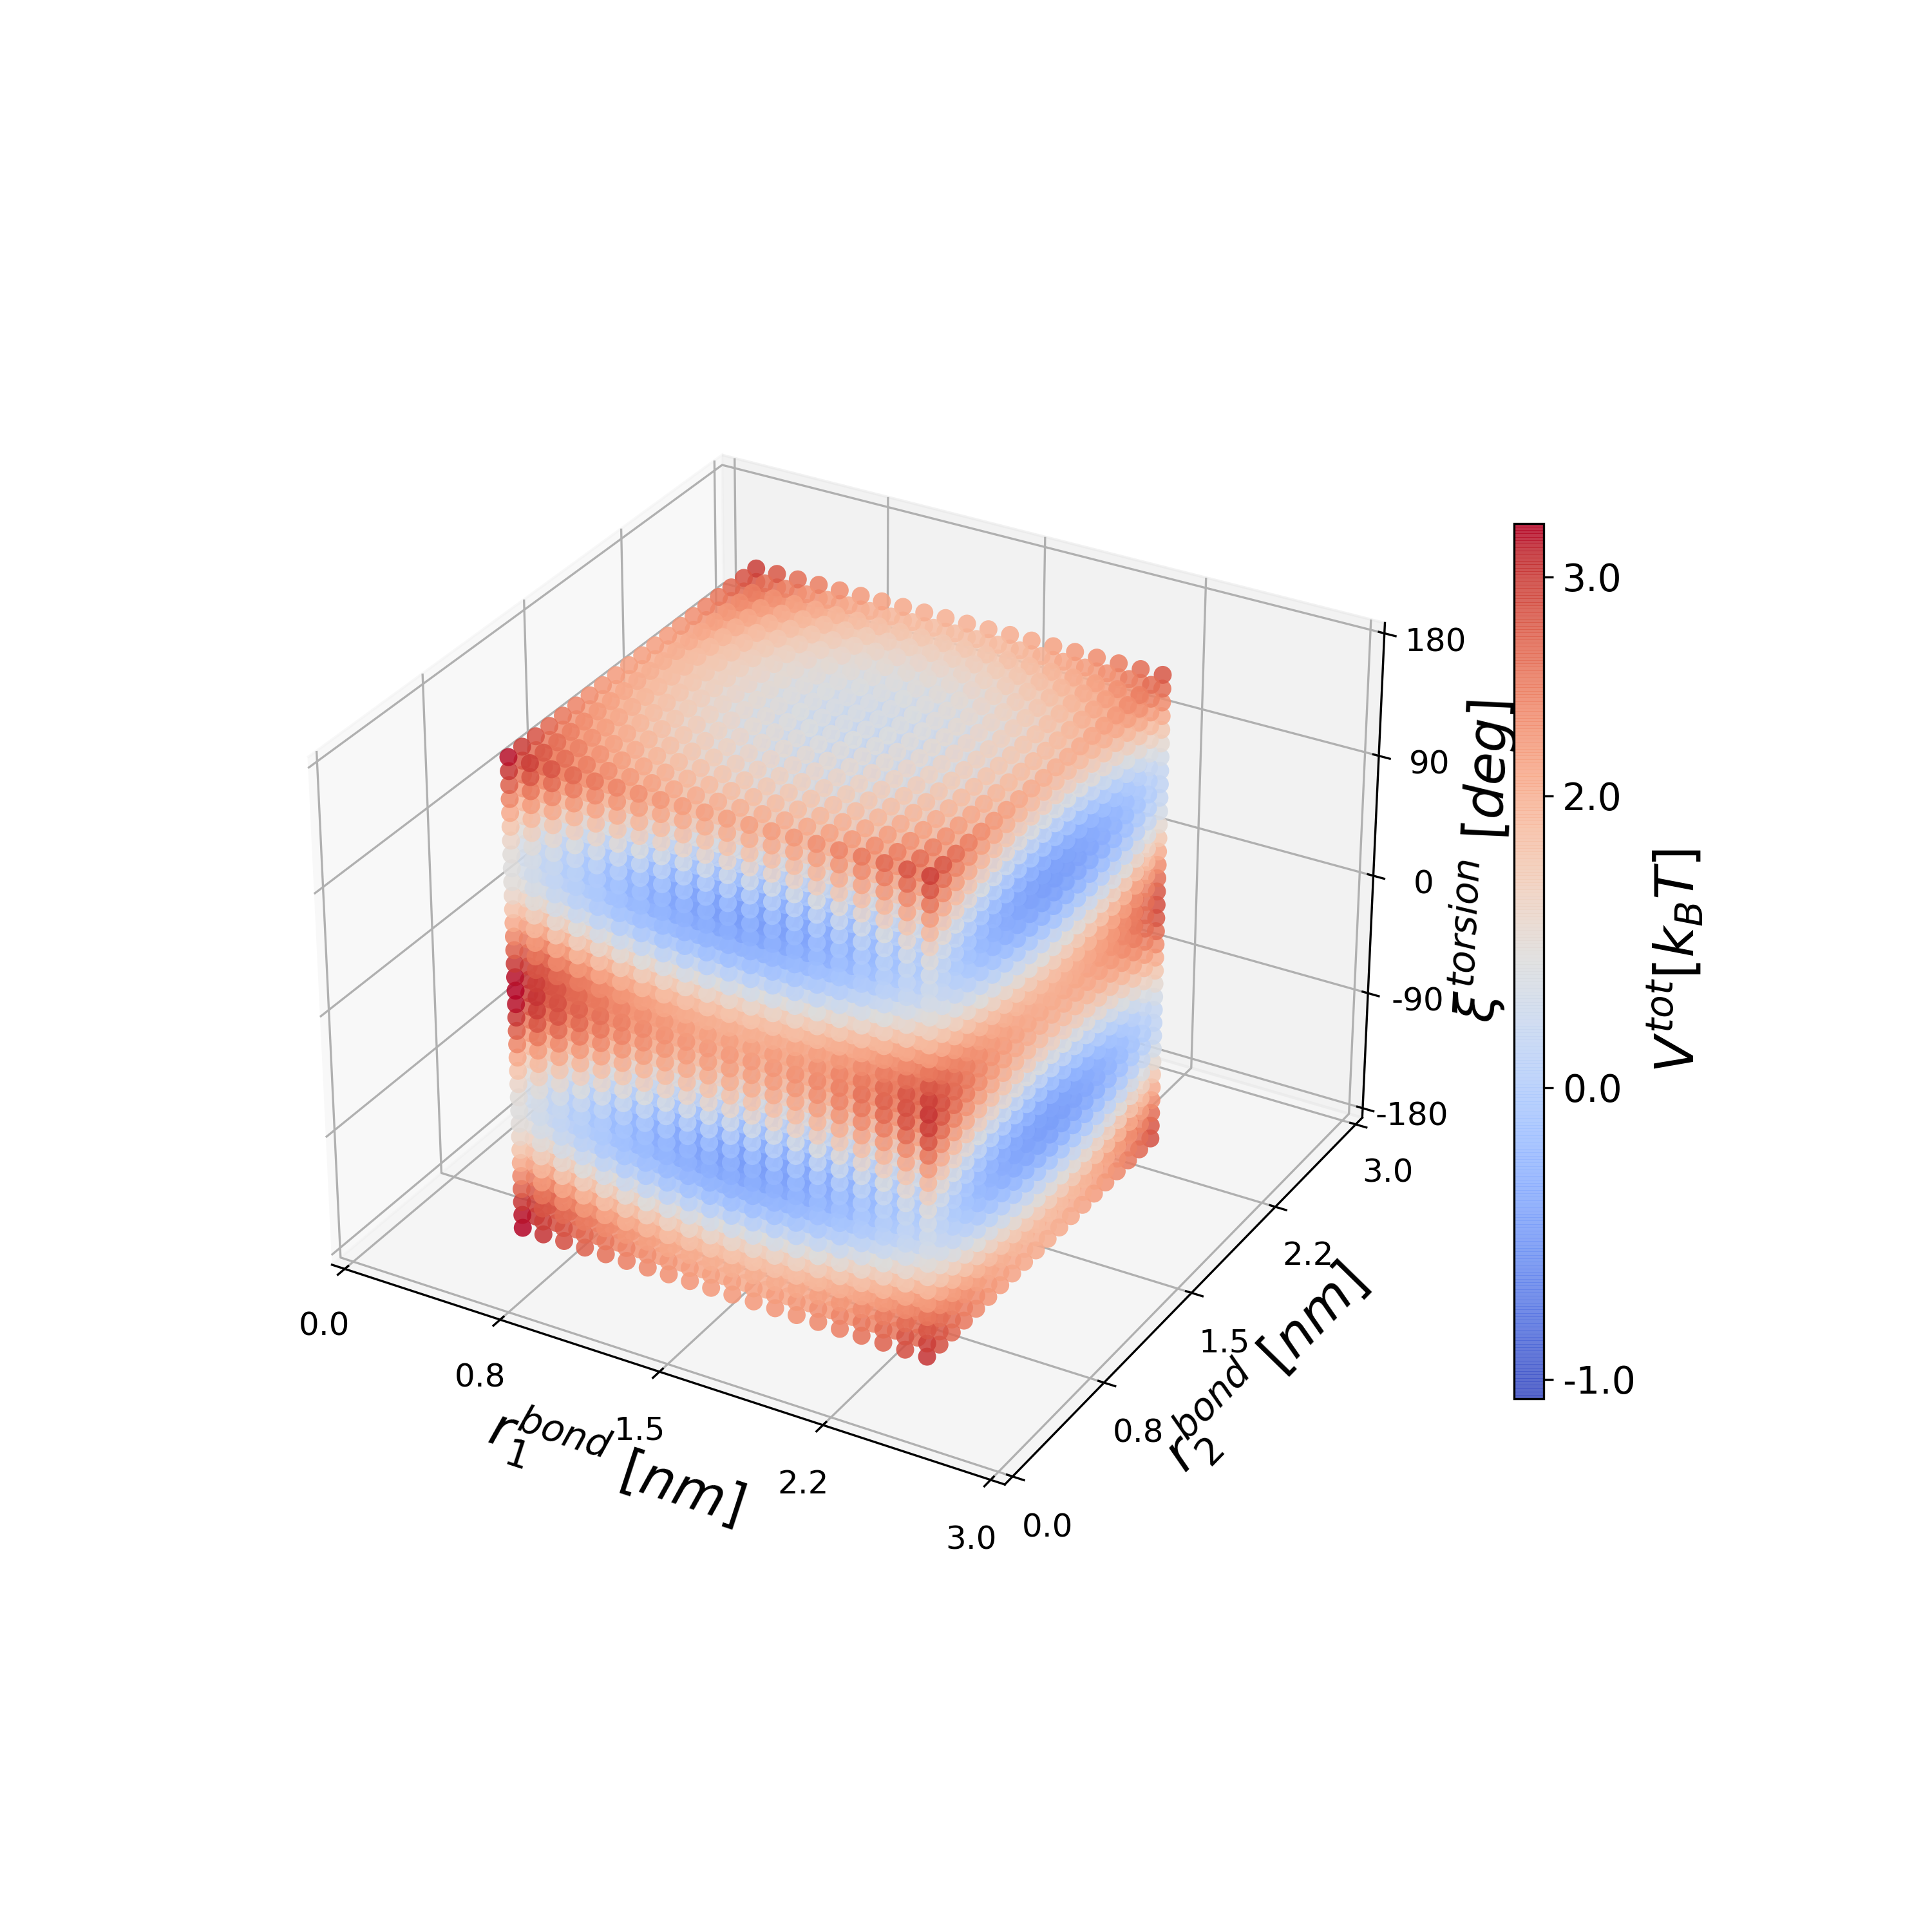
\includegraphics[width=\textwidth]{2_chapter_intro/fig/ForceField/bondterms.png}
    \caption{This PES was constructed with a grid from a FF containing two bond stretch interactions and torsion angle interaction terms of an abstract system.}
    \label{fig:ffPES}
\end{figure}

Many force fields functions and parameter sets were developed in the past,such as AMBER\cite{Weiner1981, Pearlman1995, Cornell1995, Lindorfflarsen2010}, GROMOS\cite{Daura1998, Oostenbrink2004, Schuler2001, Schmid2011,Malde2011, Stroet2018}, CHARMM\cite{Brooks1983, Mackerell1995, Mackerell1998}, OPLS \cite{Jorgensen1988, Jorgensen1996} and OpenFF \cite{Qiu2021}
Additionally, automatic molecule parametrizing tools were developed, such as the Automated Topology Builder (ATB) \cite{Malde2011, Stroet2018} or the Generalized Amber Force Field (GAFF)\cite{Sprenger2015}.

Last it should be mentioned that in practice, the bond terms are replaced for large biomolecule simulations by Lagrange multiplier-based constraint algorithms such as the SHAKE\cite{Ryckaert1977, Ciccotti1986}, SETTLE\cite{Miyamoto1992} or the LINCS\cite{Hess1997} algorithm, resulting in the omission the bond vibrations. \cite{Ryckaert1977} 
Application of such constraint algorithms allows the use of  larger timesteps up to $2~fs$, increasing the efficiency of the MD simulation. \cite{Cornell1995, Oostenbrink2004}


%%%Integration
\subsection{Integration Schemes}
Many different multi-step integration methods can be used to integrate the force field functions resulting in different outcomes for various purposes. 

One category of methods is the multi-step optimization algorithms such as the steepest descent \cite{Debye1909}, or conjugated gradient \cite{Hestenes1952} algorithms. These algorithms are used to find local minima in the PES, usually used as starting configurations in a follow-up simulation in molecular modeling.\cite{Cazals2015}
A second category of multi-step integrations methods is represented by stochastic approaches, like the Monte-Carlo approach or the Metropolis-Hastings integrator\cite{Hastings1970}, that depends on the Metropolis-Monte Carlo Criterion\cite{Metropolis1953}.  These approaches can be used to sample the PES stochastically. 
The most used category of methods for integration in MD is based on the Newtonian laws of motion\cite{Newton1726, Cohen1999}. 
Usually employed algorithms in this category are second order algorithms like the Verlet or leap-frog alrogithms \cite{Hockney1970} founded on performance and sufficient accuracy. \cite{Gunsteren1990}
Fundamentally the leap-frog algorithm works as follows,
\begin{equation}
    \begin{split}
        \textbf{r}(t+\Delta t)&=~\textbf{r}(t)+v(t+\frac{1}{2} t) \Delta t \\
        \textbf{v}(t+\frac{1}{2} \Delta t)&=~\textbf{v}(t - \frac{1}{2} \Delta t)+a(t) \Delta t \\
        \textbf{a}(t)&= \frac{F(r(t))}{m},
    \end{split}
\end{equation}
with $F(\textbf{r}(t))$ as $\partial V/ \partial \textbf{r}$ coming from the derivation of the force field function.\cite{Gunsteren1990}
This integration class gives insights not only into the sampled PES, but also in dynamics based of the PES traversal base on Netwonian laws\cite{Newton1726, Cohen1999} which are a common concept in nature.

 
%%%Conditions
\subsection{Conditions}
As the last section in this short glimpse on simulations in computational chemistry, we want to look at the additional tools that allow setting specific conditions for MD simulation approaches. 
These conditions are essential in order to correctly retrieve thermodynamic properties at certain physical conditions from the simulations, such that they can be used in the context of experimental setups. Here we will glimpse at two of the most used ensembles in the context of Newtonian integrators.

The Canonical (NVT) ensemble keeps the number of particles (N), the system box volume (V), and temperature (T) constant. Keeping N and V constant is, in most cases, trivial. In contrast, to keep T constant in a simulation, which directly is connected to the velocities of the particles,  multiple different thermostat algorithms were developed in the past. The first approach was introduced by Berendsen\cite{Berendsen1984} with the weak coupling thermostat. Because of the T/particle velocity relation in a system, the weak coupling thermostat scales the velocities by a factor $\lambda(t; \tau_T, \Delta t, T_0)$ in order to maintain the constant temperature.  
\begin{equation}
    \lambda(t; \tau_T, \Delta t, T_0) = \sqrt{1 + \frac{\Delta t}{\tau_{T}} \left( \frac{T_0}{T(t)}-1 \right) },
\end{equation}
with the coupling time parameter  $\tau_{T}$ and the reference temperature $T_{0}$.\cite{Berendsen1984}
More sophisticated approaches are the Nos\'e-Hoover\cite{Nose1984, Nose1984A, Hoover1985} or Nos\'e-Hoover chain\cite{Martyna1992} thermostat. Note that the Metropolis-Hastings algorithm leads automatically to an NVT ensemble because of the temperature given in the metropolis-monte Carlo criterion \cite{Hastings1970}. The NVT ensemble can be used to calculate Helmholtz free energies\cite{Helmholtz1882}.

The second important ensemble is the Isobaric-isothermal (NPT) ensemble with constant pressure (P). The pressure can be kept constant by barostat algorithms, like the weak coupling barostat by Berendsen\cite{Berendsen1984} functioning similar to the thermostat, Parinello-Rahman barostat\cite{Parrinello1981}, and Nos\'e-Hoover barostat\cite{Nose1983}. From an NPT ensemble a Gibbs distribution is retrieved allowing the calculation of Gibbs free energies\cite{Gibbs1879}. This ensemble is supposed to be closest to a given experimental setup at a defined pressure and temperature.

\section{Free Energies}
Free energies are elemental quantities that describe the energy of states. In chemistry, the difference of free energies is used to characterize, for example, the spontaneity of reactions, the formation of polymers, or protein-ligand binding.\cite{Kollman1993, Armacost2020, Christ2009, Hansen2014, Cournia2020} 

From thermodynamics perspective, the Helmholtz free energy\cite{Helmholtz1882} for a canoncial ensemble can be obtained as, 
\begin{equation}
    A =  -\frac{1}{\beta} \ln(Q(N, V, T)),
\end{equation}
with Q(NVT) as the partition function of the system. \cite{Atkins2014}

The canonical ensemble is Boltzmann distributed \cite{Boltzmann1872} and therefore the partition function can be formulated as,
\begin{equation}
    Q =\sum^N_i e^{-\beta E_i} ,
\end{equation} for an ensemble with discrete energy levels.  \cite{Atkins2014}

A common principle in many free-energy-based methods is to calculate the free energy difference between two end-states. \cite{Ytreberg2006, Kirkwood1935, Zwanzig1954} Examples for such end-states could be the bound and unbound states of a protein-ligand complex or the assembled and disassembled states of polymers. \cite{Kollman1993, Armacost2020, Christ2009, Hansen2014, Cournia2020} 

A free energy difference between two end-states $A$ and $B$ can be therefore defined as,  \cite{Atkins2014}
\begin{equation}
    \begin{split}
        \Delta A_{AB} &= -\frac{1}{\beta} (\ln( Q_B(N, V, T) ) - \ln(Q_A(N, V, T)))\\
        &= -\frac{1}{\beta} \ln(\frac{Q_B(N, V, T)}{Q_A(N, V, T)}).
    \end{split}
\end{equation}

The ensembles generated by MD simulations approximate the partition functions for the end-states, by sampling the hamiltonian of the system $H(\textbf{r},\textbf{p})=V(\textbf{r})+K(\textbf{p})$ over the phase space as,\cite{Zwanzig1954} 
\begin{equation}
    Q = \frac{1}{h^{3N} N!}  \int \int e^{-\beta H(\textbf{p},\textbf{r})} d \textbf{p} d \textbf{r} ,
\end{equation}
for indistinguishable particles with $h$ as Planck constant and $N$ the number of particles.\cite{Zwanzig1954}

From this, the Zwanzig equation\cite{Zwanzig1954} can be derived by using the Boltzmann factors ($p=-\frac{e^{-\beta V_x}}{\sum^N e^{-\beta V_x}}$) of the two end-states $A$ and $B$ sampled as the ensemble Average over state A \cite{Zwanzig1954}, 
\begin{equation}
        \Delta A_{AB} 
        = -\frac{1}{\beta} \ln\langle \frac{e^{-\beta V_B}}{e^{-\beta V_A}}\rangle_A
        = -\frac{1}{\beta} \ln\langle e^{-\beta V_B-V_A}\rangle_A .
\end{equation}
In the chapters \ref{ch:feens}-\ref{ch:fereeds} multiple free energy calculation methods will be discussed, further developed and applied. 